\documentclass[a0paper,portrait]{baposter}



\usepackage{wrapfig}
\usepackage{lmodern}

\usepackage[utf8]{inputenc} %unicode support
\usepackage[T1]{fontenc}

\usepackage{graphicx} % Allows including images
\usepackage{booktabs} % Allows the use of \toprule, \midrule and \bottomrule in tables
\usepackage{amsmath}
\usepackage{amsfonts}
\usepackage{ifthen}
\usepackage{amssymb}
\usepackage{amsbsy}
\usepackage{bm}
\usepackage{ulem}
\usepackage{float}
\usepackage{latexsym}
\usepackage{comment}
\usepackage{graphicx}
\usepackage{amstext}
\usepackage{latexsym}
\usepackage{arydshln}
\usepackage{longtable}
\usepackage{enumerate}
\usepackage{multirow}
\usepackage{cases}
\usepackage{geometry}
\usepackage{mathtools}
\usepackage{subeqnarray}
\usepackage{textcomp}
\usepackage[hidelinks]{hyperref}
%\usepackage{subfigure}
\usepackage{url}
\usepackage{threeparttable}
\usepackage{xr}
\usepackage{multirow}
\usepackage{wrapfig}
\usepackage{lscape}
\usepackage{rotating}
\usepackage{subcaption}
\usepackage{epstopdf}
\usepackage{verbatim}
\usepackage{xcolor}
\usepackage[sort&compress]{natbib}



\selectcolormodel{cmyk}

\graphicspath{{figures/}} % Directory in which figures are stored




\newcommand{\bA}{\mathbf{A}}
\newcommand{\bB}{\mathbf{B}}
\newcommand{\bD}{\mathbf{D}}
\newcommand{\bF}{\mathbf{F}}
\newcommand{\bI}{\mathbf{I}}
\newcommand{\bLambda}{{\bm\Lambda}}
\newcommand{\bOmega}{{\bm\Omega}}
\newcommand{\bM}{\mathbf{M}}
\newcommand{\bN}{\mathbf{N}}
\newcommand{\bphi}{{\bm\phi}}
\newcommand{\bpsi}{{\bm\psi}}
\newcommand{\brho}{{\bm\rho}}
\newcommand{\bvarphi}{{\bm\varphi}}
\newcommand{\bW}{\mathbf{W}}
\newcommand{\sT}{\mathrm{T}}
\newcommand{\bZ}{\mathbf{Z}}
\newcommand{\shalf}{\mbox{{\footnotesize$\frac{1}{2}$}}}
\newcommand{\red}[1]{\textcolor{red}{#1}}



\newcommand{\compresslist}{%
\setlength{\itemsep}{0pt}%
\setlength{\parskip}{1pt}%
\setlength{\parsep}{0pt}%
}

\newenvironment{boenumerate}
  {\begin{enumerate}\renewcommand\labelenumi{\textbf\theenumi.}}
  {\end{enumerate}}



\begin{document}


\definecolor{darkred}{RGB}{200, 16, 26}
\definecolor{lightred}{RGB}{250,100,100}
\definecolor{blue1}{RGB}{51,51,255}
\definecolor{blue2}{RGB}{127,0,255}
\definecolor{blue3}{RGB}{51,153,255}







\begin{poster}
{
grid=false,
headerborder=open, % Adds a border around the header of content boxes
colspacing=1em, % Column spacing
bgColorOne=white, % Background color for the gradient on the left side of the poster
bgColorTwo=white, % Background color for the gradient on the right side of the poster
borderColor=darkred, % Border color
headerColorOne=lightred, % Background color for the header in the content boxes (left side)
headerColorTwo=lightred, % Background color for the header in the content boxes (right side)
headerFontColor=white, % Text color for the header text in the content boxes
boxColorOne=white, % Background color of the content boxes
textborder=rounded, %rectangle, % Format of the border around content boxes, can be: none, bars, coils, triangles, rectangle, rounded, roundedsmall, roundedright or faded
eyecatcher=false, % Set to false for ignoring the left logo in the title and move the title left
headerheight=0.11\textheight, % Height of the header
headershape=rounded, % Specify the rounded corner in the content box headers, can be: rectangle, small-rounded, roundedright, roundedleft or rounded
headershade=plain,
headerfont=\Large\textsf, % Large, bold and sans serif font in the headers of content boxes
%textfont={\setlength{\parindent}{1.5em}}, % Uncomment for paragraph indentation
linewidth=2pt % Width of the border lines around content boxes
}
{}
%
%----------------------------------------------------------------------------------------
%	TITLE AND AUTHOR NAME
%----------------------------------------------------------------------------------------
%
{\textsf %Sans Serif
{A Hierarchical Spatial Finlay-Wilkinson Model for Analysis of Multi-Environment Field Trials
}
} 
{\sf\vspace{0.5em}\\
\textbf{Xingche Guo*, Somak Dutta, Dan Nettleton}
\vspace{0.1em}\\
Department of Statistics, Iowa State University
}
{
\includegraphics[width=45mm]{isu_logo.jpg}} % University/lab logo



%%%%%%%%%%%%%%%
\headerbox{Objective}{name=objective, column=0,row=0, span=1}{
\begin{itemize}
\item  Create a multidisciplinary framework for understanding and managing crop performance over \textcolor{blue3}{diverse environmental conditions.}
\item Incorporate \textcolor{blue3}{spatial effects}, \textcolor{blue3}{genetic}, and \textcolor{blue3}{environmental information} to enhance understanding of genomes-by-environment (GxE) interaction.
\item Distinguish corn varieties that are highly \textcolor{blue3}{adaptable} to changing environments.
\item \textcolor{blue3}{Predict} the yield of a (possibly novel) corn variety in a (possibly new) environment.
\end{itemize}

}




%%%%%%%%%%%%%%%
\headerbox{Data Introduction}{name=data, column=0, below=objective, span=1}{


\includegraphics[width=70mm]{g2f_logo}

We only focus on 2015 G2F dataset with: 

\begin{itemize}
	\item A subset of 24 \textcolor{blue3}{environments} (field trials).
	\item Yield recorded for 10,971 \textcolor{blue3}{field plots} with known \textcolor{blue3}{spatial locations}.
	\item A total of 1,105 \textcolor{blue3}{hybrid genotypes} (varieties).  
	\item \textcolor{blue3}{SNPs sequence} data at $\sim$1M genomic loci are available.
	\item  Time-indexed measurements for \textcolor{blue3}{weather variables} (temperature, rainfall amount, solar radiation, etc), and several \textcolor{blue3}{soil variables} (pH value, soil organic matter, etc).
\end{itemize}

}





%%%%%%%%%%%%%%%%
\headerbox{Finlay-Wilkinson (FW) Model}{name=model1, column=1, row=0, span=2}{
\begin{itemize}
\item FW model \citep{finlay1963analysis}: 
$y_{ijk} = \mu + g_i + h_j + b_i h_j + e_{ijk}$, \\
where $\mu$ is the overall mean, 
$g_i$ is the \textcolor{blue3}{genotype} effect, $h_j$ is the \textcolor{blue3}{environment} effect, $ b_i h_j$ is the FW-type multiplicative \textcolor{blue3}{interaction} effect.
\end{itemize}

\vspace{-1.5em}
  \begin{figure}[H]
  \begin{subfigure}{0.49\textwidth}
    \centering
    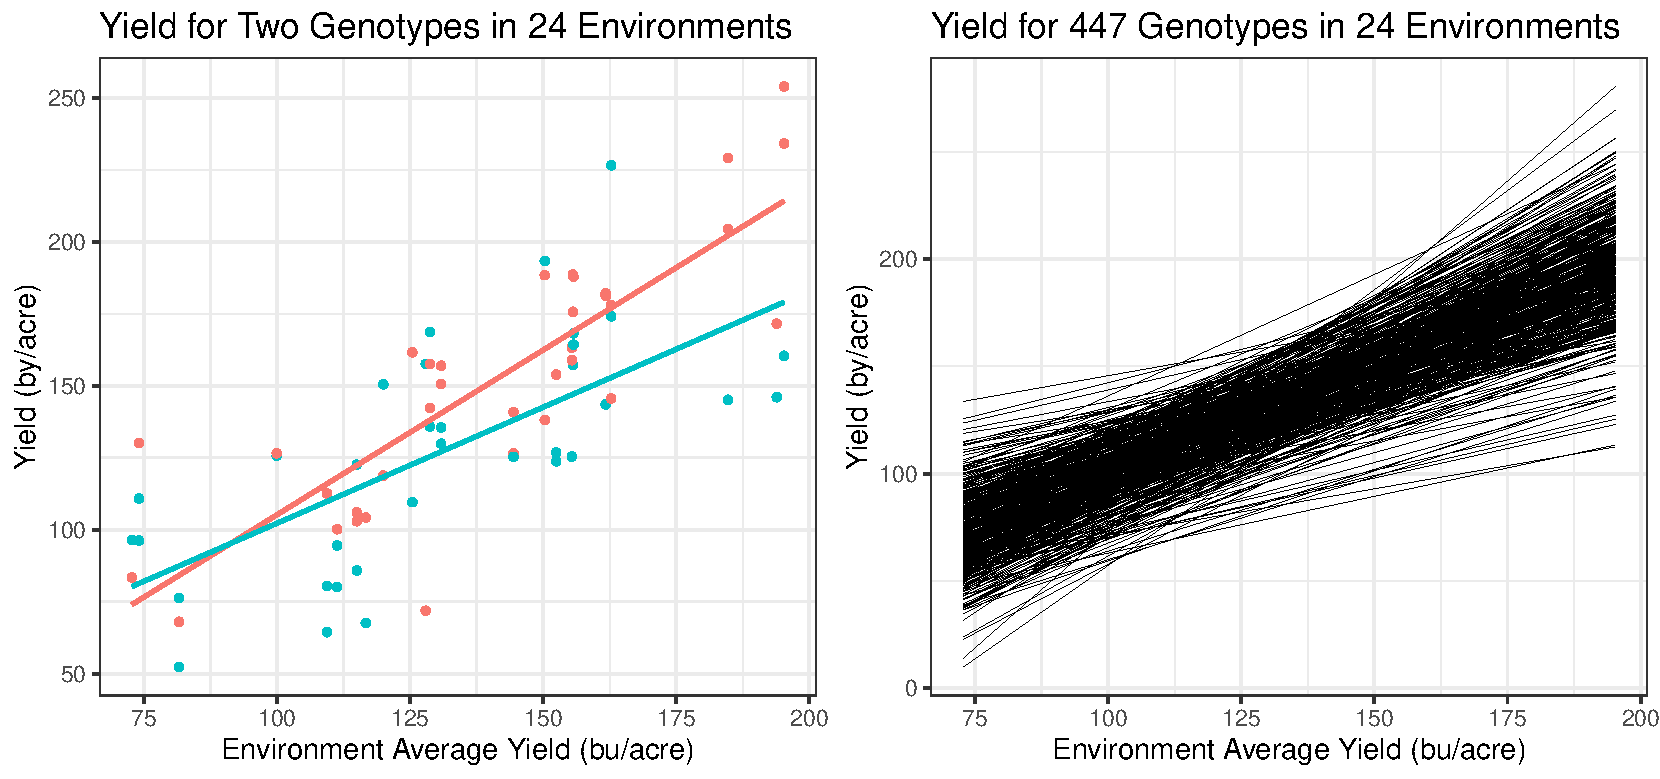
\includegraphics[width=0.95\linewidth]{fw_plot_paper.pdf}
    \vspace{-0.5em}
    \caption{\scriptsize{ \textit{ \textbf{FW Model Mechanism Diagram}: Left panel: the scatterplot of yield versus environment average yield for 24 field trials and
the fitted FW lines for two example corn varieties using 2015 G2F data; Right panel: the fitted FW lines for 447 example corn varieties.}} }
  \end{subfigure}
  \begin{subfigure}{0.48\textwidth}
    \centering
    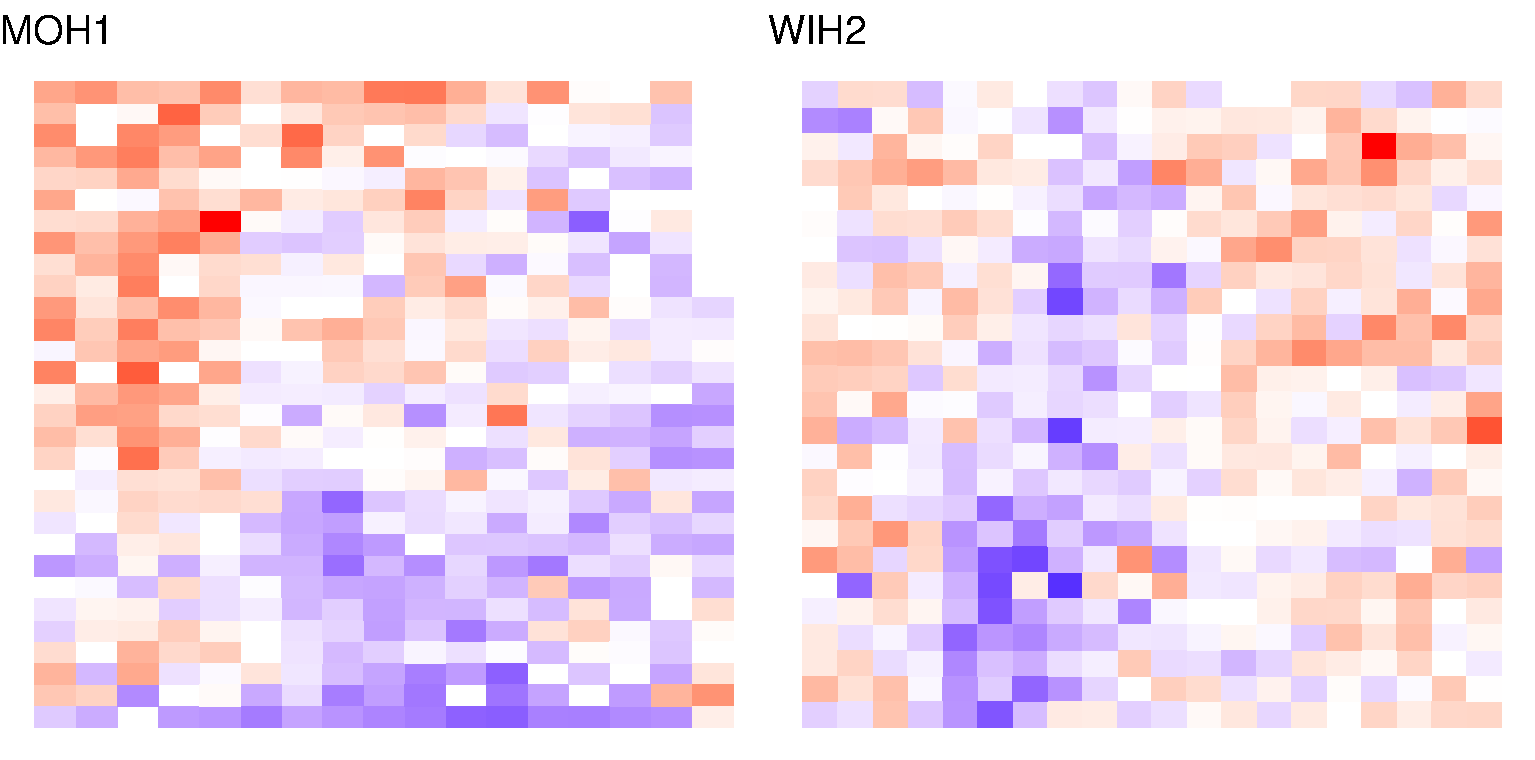
\includegraphics[width=0.95\linewidth]{resid_plot_2.pdf}
    \vspace{-0.5em}
    \caption{ \scriptsize{ \textit{ \textbf{Residuals of FW Model for Two Fields}: 
     The rectangular plots in the fields are colored based on the value of the residuals. We find that there are clear color patterns in the fields, which means the residuals are highly spatially correlated.}} }
  \end{subfigure}
  \end{figure}

}




%%%%%%%%%%%%%%%%%
\headerbox{Hierarchical Spatial Finlay-Wilkinson (HSFW) Model}{name=model2, column=1, below=model1, span=2}{

\begin{itemize}
\item Data model:
$[y_{ijk} | \mu, \mathbf{g}, \mathbf{b}, \mathbf{h}, \red{\bphi} ] \ \ \overset{indep}{\sim} \ \  \mathcal{N}(\mu + g_i + h_j + b_i h_j + \red{\phi_{ijk}}, \sigma_e^2)$.

\item Prior distributions for \textcolor{blue3}{genotype}, \textcolor{blue3}{slope}, and \textcolor{blue3}{environment} effects:
$$  [\mathbf{g}] \sim \mathcal{N}(\bm{0}, \bA \sigma_g^2); \ \ \ \ \ \ \ [\mathbf{b}] \sim \mathcal{N}(\bm{0}, \bA \sigma_b^2); \ \ \ \ \ \ \ \ [\mathbf{h}|\bm{\gamma}] \sim \mathrm{N}( \gamma_1 \bZ_1 +  \dots + \gamma_L \bZ_L, \mathbf{I} \sigma_h^2).$$
$\bA$ is the kinship matrix describing the correlation structure between different hybrid corn varieties; $\bZ_{l}$ is the $l$th standardized environmental covariate.

\item First order intrinsic autoregression (IAR) prior for \textcolor{blue3}{spatial} effects: \citep{besag1999bayesian,dutt:mond:2015}.
\begin{equation*}
[\bpsi_j|\theta_j,\sigma^2_j] \propto |\sigma^{-2}_j\bW_j|_+^{1/2}\exp\left( -\shalf\sigma^{-2}_j\bpsi_j^\sT \bW_j\bpsi_j\right),
\end{equation*}
where
\[\bpsi_j^\sT \bW_j\bpsi_j = \theta_j\sum\sum(\psi_{u,v} - \psi_{u-1,v})^2 + {\bar\theta}_j\sum\sum(\psi_{u,v} - \psi_{u,v-1})^2.\]

\item Projected intrinsic autoregression (PIAR) prior (A \textcolor{blue3}{sum-to-zero} constrained version of IAR prior):
\begin{equation*}
\bphi_j = \bB_j \bvarphi_j,\qquad \bvarphi_j\sim{\mathcal N}(\mathbf{0},\bD_j^{-1}),
\end{equation*}
$\bD_j$ is the diagonal matrix with its diagonal entries to be all the \textcolor{blue3}{nonzero eigenvalues} of $\bW_j$; $\bB_j$ is the corresponding \textcolor{blue3}{eigenvector} matrix. We develop \textcolor{blue3}{matrix free algorithm} for the fast computation.

\item Implement posterior predictive distributions for: (i) \textcolor{blue3}{within-field prediction}; (ii) \textcolor{blue3}{prediction in new environments}. \textcolor{blue3}{Prediction intervals} can also be obtained.

\end{itemize}

}





%%%%%%%%%%%%%%%%%
\headerbox{Data Analysis}{name=analysis, span=2, column=1, below=model2, above=bottom}{ % To reduce this block to 1 column width, remove 'span=2'

\vspace{-0.5em}
 \begin{figure}[H]
%  \begin{subfigure}{0.55\textwidth}
%    \centering
%    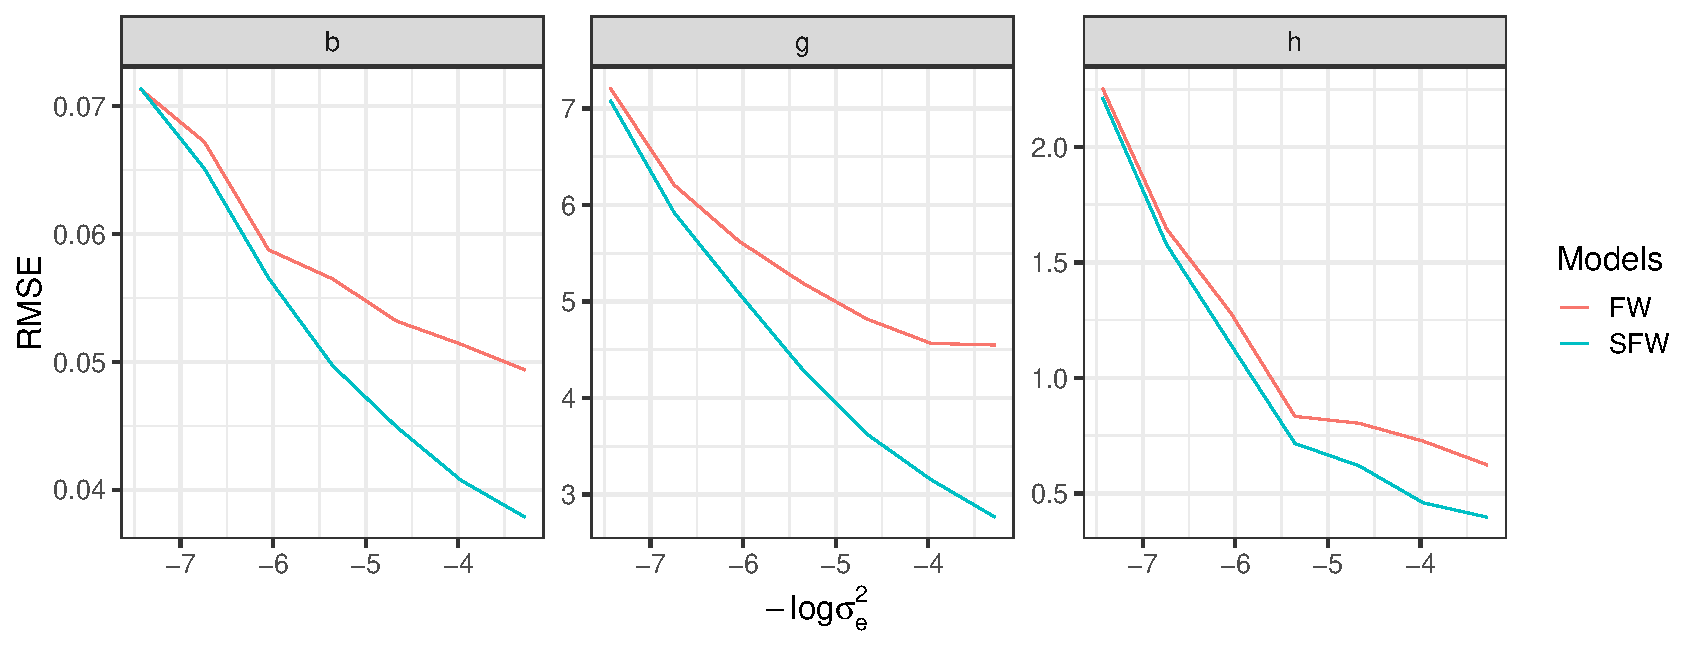
\includegraphics[width=0.95\linewidth]{com_simu_gbh2.pdf}
%    \caption{Model Evaluation via Simulation Study: The averaged RMSEs of genotype, slope, and field effects versus different signal-noise ratio levels under FW and SFW model.}
%  \end{subfigure}
  \begin{subfigure}{0.49\textwidth}
    \centering
    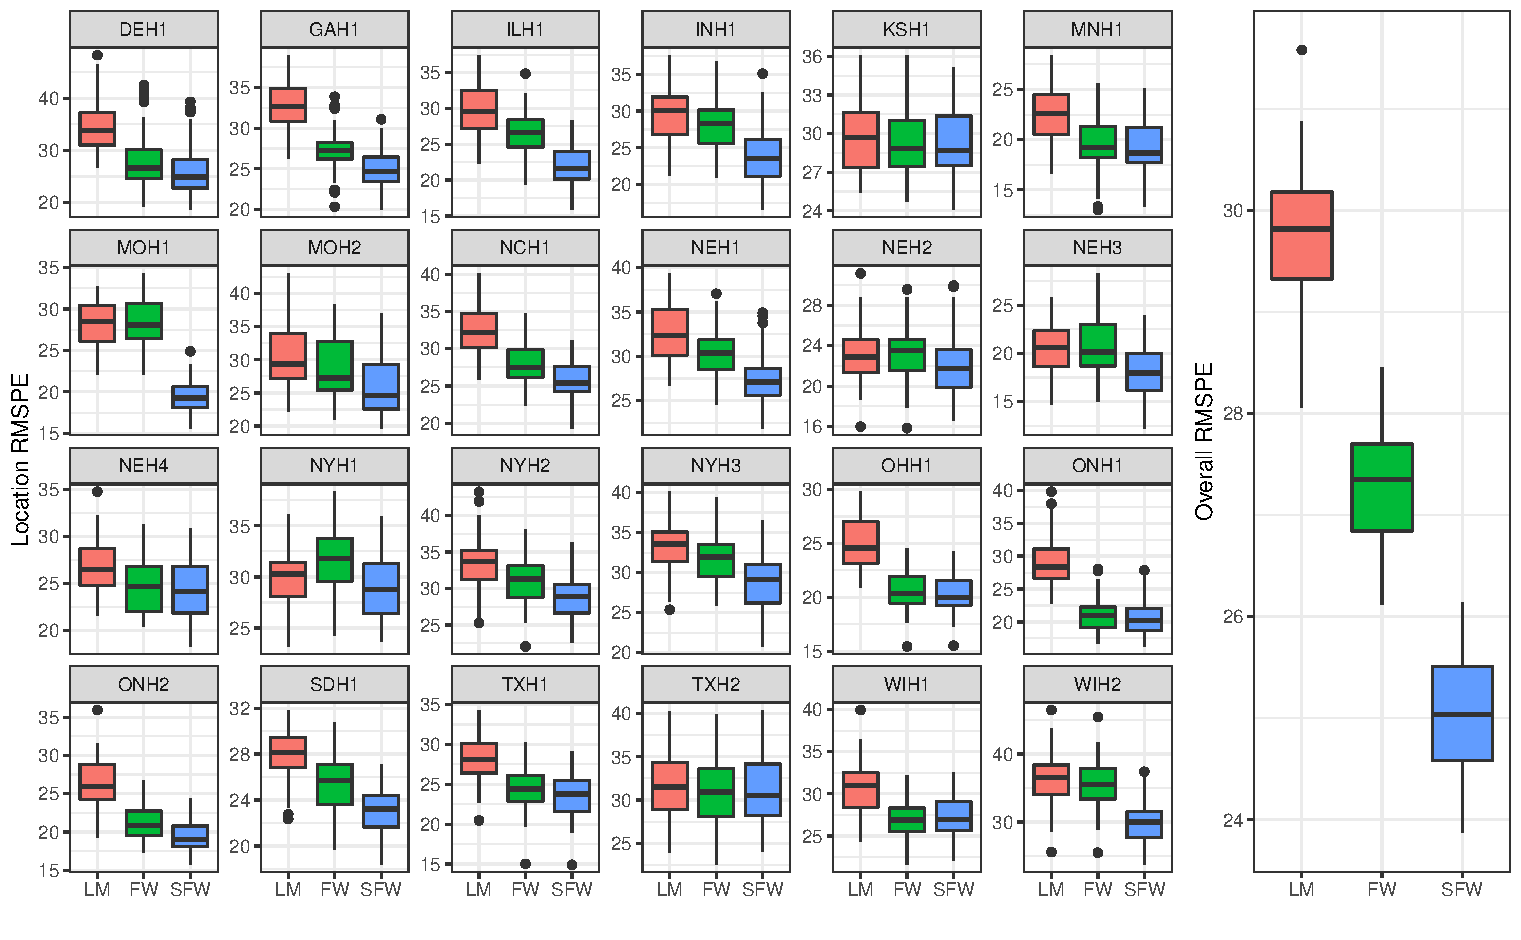
\includegraphics[width=0.95\linewidth]{com_pred3.pdf}
    \vspace{-0.5em}
    \caption{ \scriptsize{ \textit{ \textbf{Model Evaluation via Within-Field Prediction}: Left panel: location-wise RMSPE computed by linear additive model (LM), Finlay-Wilkinson model (FW), and Finlay-Wilkinson model with spatial effects (SFW); Right Panel: overall RMSPE computed by these three models.} } }
  \end{subfigure}
  \begin{subfigure}{0.47\textwidth}
    \centering
    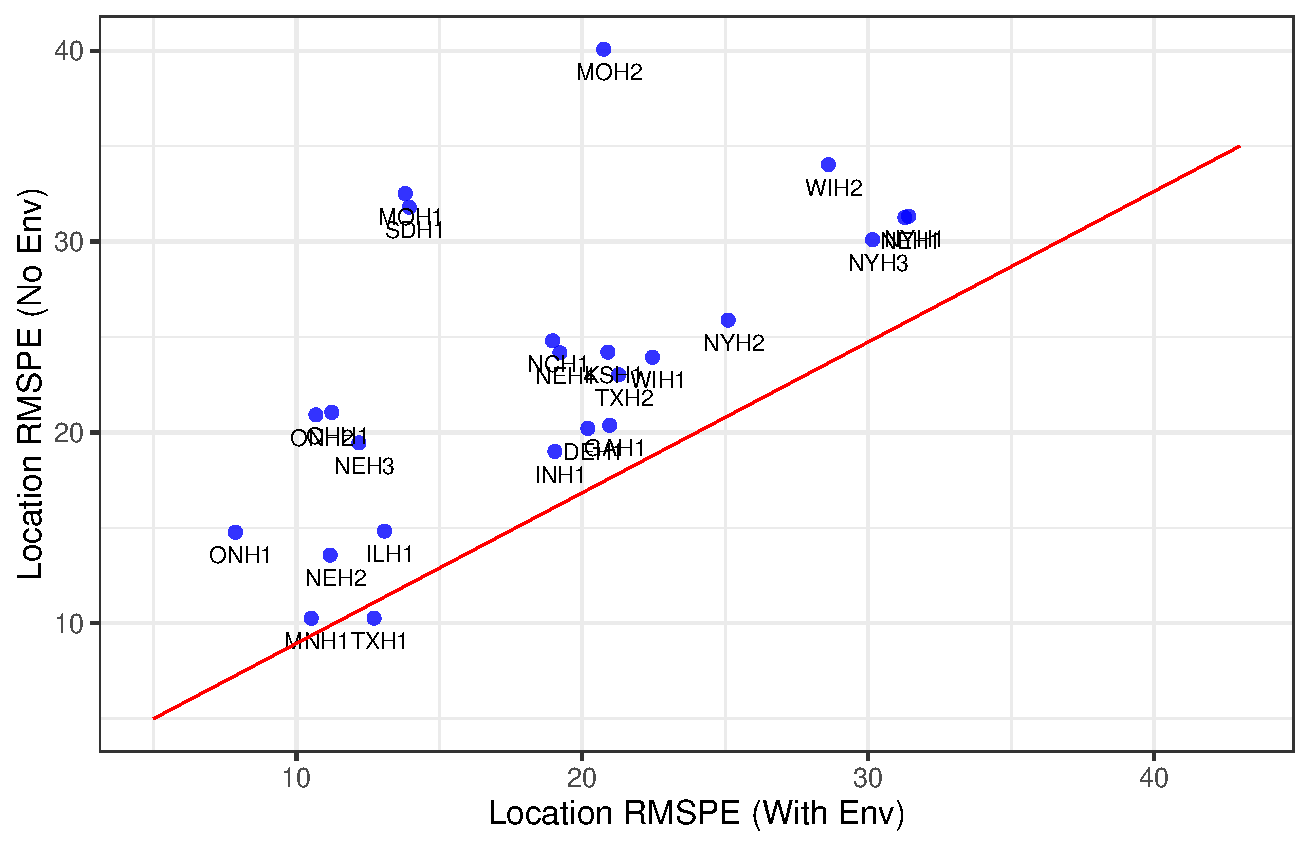
\includegraphics[width=0.95\linewidth]{type3pred1.pdf}
    \vspace{-0.5em}
    \caption{  \scriptsize{ \textit{ \textbf{Predict in New Environments}: The scatterplot of the 24 location-wise RMSPEs computed using temperature and rainfall data ($x$-axis), versus the location-wise RMSPEs computed not using any environment information ($y$-axis).}} }
  \end{subfigure}
%
%
%  \begin{subfigure}{0.45\textwidth}
%    \centering
%    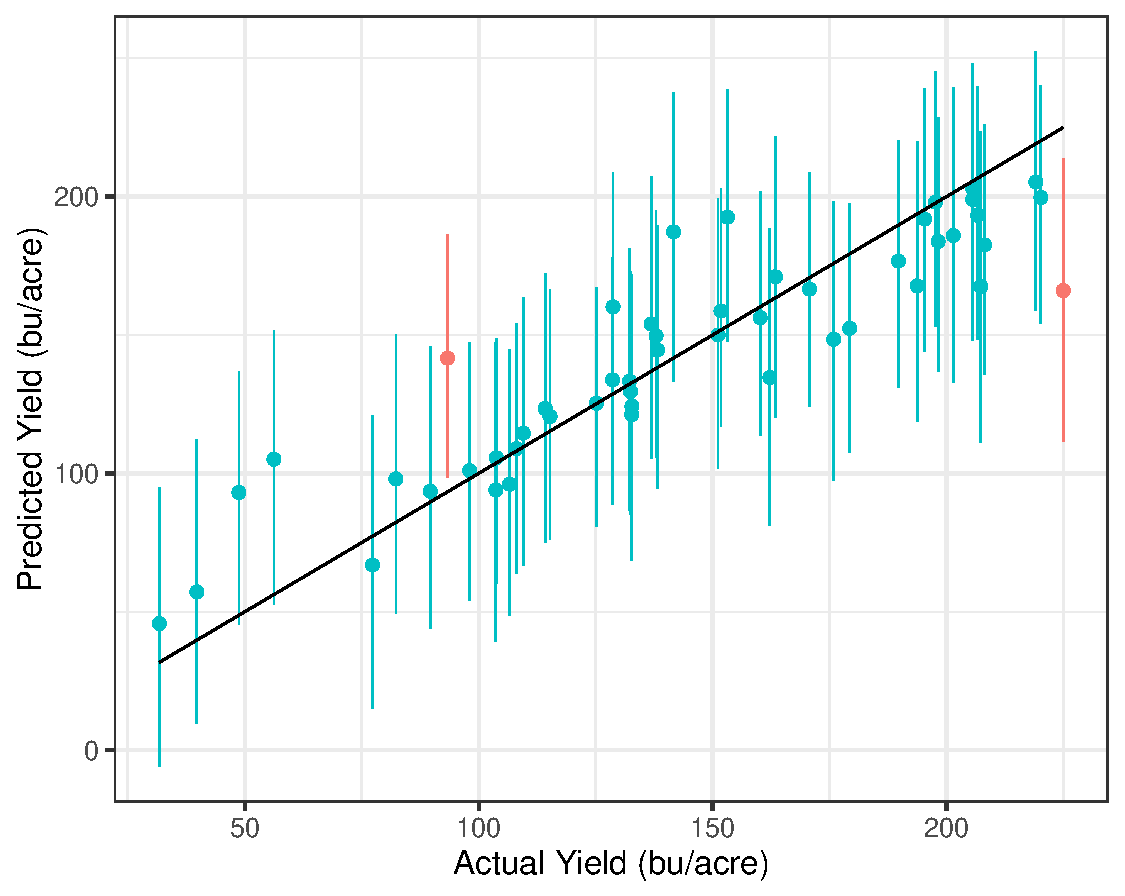
\includegraphics[width=0.9\linewidth]{true_vs_predint.pdf}
%    \caption{Prediction Intervals.}
%      \end{subfigure}
  \end{figure}
 
 
\vspace{-1.5em}
\begin{table}[H]
\scalebox{0.9}{
\begin{tabular}{ccccccc}
\hline
 & \multicolumn{3}{c}{\ \ \ \ \ \ \ \  $90\%$ CL} &  \multicolumn{3}{c}{\ \ \ \ \ \ \ \ $95\%$ CL}   \\
 &  \ \ \ \ \ \ \ \ LM  &  FW  &  SFW &  \ \ \ \ \ \ \ \ LM  &  FW  &  SFW  \\
\hline
Coverage Percentages  &  \ \ \ \ \ \ \ \  90.3\%   & 89.9\%   & 90.1\% & \ \ \ \ \ \ \ \  95.3\%  &  94.9\%   & 94.5\%     \\          
Median Interval Widths   & \ \ \ \ \ \ \ \  98.4 & 90.3 &  80.1  & \ \ \ \ \ \ \ \  117.3   &  107.5  & 95.76    \\ 
\hline
\end{tabular}
}
\vspace{-0.5em}
\caption*{ \scriptsize{ \textit{ \textbf{Compare Prediction Interval Widths}: the median credible interval widths of LM, FW, and SFW models at $90\%$ and $95\%$ credible levels are provided. SFW model has a more precise interval prediction given that SFW model has the shortest interval widths at the same coverage levels.
}} }

\end{table}

 
 
  
}





%%%%%%%%%%%%%%%%%
\headerbox{Future Work}{name=future, span=1, column=0, below=data}{ % To reduce this block to 1 column width, remove 'span=2'

\begin{itemize}
\item Allow \textcolor{blue3}{more complex models} (non-linear models, time series models, functional data models, etc) for environmental covariates.
\item Formulate better \textcolor{blue3}{kinship matrix} to improve estimation and further accelerate the algorithm.
\item Extend to \textcolor{blue3}{generalized} HSFW model to account for \textcolor{blue3}{discrete} value responses.
\end{itemize}

}





%%%%%%%%%%%%%%%%%
\headerbox{References}{name=references, column=0, span=1, below=future}{

%\small % Reduce the font size in this block
\renewcommand{\section}[2]{\vskip 0.05em} % Get rid of the default "References" section title
%\nocite{*} % Insert publications even if they are not cited in the poster

\bibliographystyle{apalike}
 \scriptsize{\bibliography{FWspatial}} % Use sample.bib as the bibliography file
}







%%%%%%%%%%%%%%%%%
\headerbox{Acknowledgements}{name=acknowledgements, column=0, span=1, below=references, above=bottom}{

 \tiny{The authors acknowledge financial support of \textcolor{blue1}{Iowa State University Plant Sciences Institute Scholars Program}, the \textcolor{blue1}{Baker Center for Bioinformatics and Biological Statistics}, and the \textcolor{blue1}{Iowa Agriculture and Home Economics Experiment Station}, Ames, Iowa, Project \textcolor{blue2}{No. IOW03617}, which is supported by \textcolor{blue1}{USDA/NIFA} and \textcolor{blue1}{State of Iowa} funds.}

}

\end{poster}




\end{document}
